\chapter{Echtzeitbetriebssysteme}
\section{Arten von Echtzeit}
\begin{itemize}
    \item Harte Echtzeit: Die Aufgabe muss zwingend vor der Deadline abgearbeitet sein
    \item Fest Echtzeit: Wenn die Information nach der Deadline kommen sind sie irrelevant
    \item Weiche Echtzeit: Die Aufgabe sollte meistens vor der Deadline abgearbeitet sein
\end{itemize}

\section{Aufgaben eines (Echtzeit-)Betriebssytems}
Standardaufgaben eines Betriebssytems:
\begin{itemize}
    \item Taskverwaltung
    \item Betriebsmittelverwaltung
    \item Interprozesskommunikation
    \item Synchronisationsaufgaben
    \item Schutzmaßnahmen
\end{itemize}
Ein Echtzeitbetriebssysteme (RTOS) muss zudem folgende Aufgaben erfüllen:
\begin{itemize}
    \item Rechtzeitigkeit
    \item Gleichzeitigkeit
    \item Verfügbarkeit
\end{itemize}

\section{Aufbau}
Ein (Echtzeit-)Betriebssytem ist normalerweise in einem Schichtenmodell aufgebaut.
\begin{figure}[H]
    \centering
    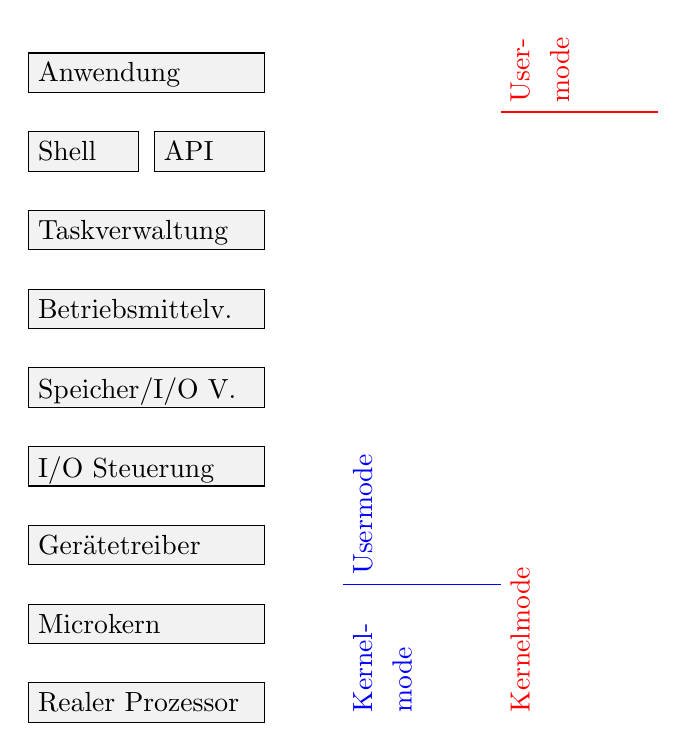
\begin{tikzpicture}
        \filldraw [draw=black,fill=gray!10] (3,0) rectangle (0,0.5) node [below right] {Realer Prozessor};
        \filldraw [draw=black,fill=gray!10] (3,1) rectangle (0,1.5) node [below right] {Microkern};
        \filldraw [draw=black,fill=gray!10] (3,2) rectangle (0,2.5) node [below right] {Gerätetreiber};
        \filldraw [draw=black,fill=gray!10] (3,3) rectangle (0,3.5) node [below right] {I/O Steuerung};
        \filldraw [draw=black,fill=gray!10] (3,4) rectangle (0,4.5) node [below right] {Speicher/I/O V.};
        \filldraw [draw=black,fill=gray!10] (3,5) rectangle (0,5.5) node [below right] {Betriebsmittelv.};
        \filldraw [draw=black,fill=gray!10] (3,6) rectangle (0,6.5) node [below right] {Taskverwaltung};
        \filldraw [draw=black,fill=gray!10] (3,7) rectangle (1.6,7.5) node [below right] {API};
        \filldraw [draw=black,fill=gray!10] (1.4,7) rectangle (0,7.5) node [below right] {Shell};
        \filldraw [draw=black,fill=gray!10] (3,8) rectangle (0,8.5) node [below right] {Anwendung};
        \draw [draw=blue] (4,1.75) -- (6,1.75);
        \node[below right,rotate=90, text=blue] at (4,0) (){Kernel-};
        \node[below right,rotate=90, text=blue] at (4.5,0) (){mode};
        \node[below right,rotate=90, text=blue] at (4,1.75) (){Usermode};
        \draw [draw=red] (6,7.75) -- (8,7.75);
        \node[below right,rotate=90, text=red] at (6,0) (){Kernelmode};
        \node[below right,rotate=90, text=red] at (6,7.75) (){User-};
        \node[below right,rotate=90, text=red] at (6.5,7.75) (){mode};
    \end{tikzpicture}
    \caption{Beispielhafter Aufbau eines Betriebssytems (Microkernel in \textcolor{blue}{blau}, Makrokernel/Monolithischer Kernel in \textcolor{red}{rot})}
\end{figure}

\section{Unterbrechungen}
\todo{Grafik, was auch immer die Aussagt?}

\subsection{Folgen von Unterbrechungen}
Es gibt nicht unterbrechbare Funktionen (\glqq{}non-reentrant\grqq{}), z.B. (\lstinline[style=c]{tmp} ist hier global):
\begin{lstlisting}[style=c]
    void swap(int *x, int *y) {
        tmp = *x;
        *x = *y;
        *y = tmp;
    }
\end{lstlisting}
Mögliche Lösungen:
\begin{itemize}
    \item \lstinline[style=c]{tmp} lokal definieren
    \item Interrupts für Funktion deaktivieren (kritisch)
    \item \lstinline[style=c]{tmp} schützen
\end{itemize}

Die meisten Funktionen sind unterbrechbar, z.B.:
\begin{lstlisting}[style=c]
    void strcpy(char *dst, const char *src) {
        while (*dst++ = *src++);
        *dst = '\0';
    }
\end{lstlisting}

\section{Taskverwaltung}
Ein Task (\glqq{}Rechenprozess\grqq{}) ist ein ablaufendes Programm zusammen mit Variablen und Betriebsmitteln.
Tasks besitzen:
\begin{itemize}
    \item Aktionsfunktionen (\glqq{}Programm\grqq{})
    \item Zustandsvariablen (Speicher, Register, PC)
\end{itemize}
\todo{Grafik}
\subsection{Taskzustände}
\begin{figure}[H]
    \centering
    \includegraphics[width=\textwidth]{taskzustande.pdf}
    \caption{Zustandsmaschine der Taskübergänge}
\end{figure}

\subsection{Taskscheduler}
\paragraph{Taskscheduler} Welcher Task soll ausgeführt werden?
\paragraph{Taskdispatcher} Notwendigen Abläufe um Task zur Ausführung zu bringen

Sobald mehr als ein Task benötigt wird muss ein Scheduler genutzt werden.
\begin{figure}[H]
    \centering
    \includegraphics[width=\textwidth]{scheduling.pdf}
    \caption{Übersicht über mögliche Scheduling-Verfahren}
\end{figure}

\subsubsection{Polled-Loop-Systeme}
Der einfachst mögliche RT-Kernel:
\begin{lstlisting}[style=c]
    int main(void) {
        while (true) {
            if (event) {
                event = false;
                threadCall(threadPtr);
            }
        }
    }
\end{lstlisting}
Nachteile: Nur ein thread kann verwaltet werden, bei Burst-Nachrichten (mehrere Nachrichten während der Thread läuft) wird nur eine abgearbeitet, Verschwendung von CPU-Zeit.

\subsubsection{Polled-Loop für mehrere Tasks}
\begin{lstlisting}[style=c]
    int main(void) {
        while (true) {
            if (event1) {
                event1 = false;
                threadCall(thread1Ptr);
            }
            if (event2) {
                event2 = false;
                threadCall(thread2Ptr);
            }
            if (event3) {
                event3 = false;
                threadCall(thread3Ptr);
            }
        }
    }
\end{lstlisting}
Gleiche Probleme wie oben (Burst). Zusätzlich kann ein Thread alle anderen aushungern.

\subsubsection{Phase-/State-Driven Systems}
\begin{lstlisting}[style=c]
    void isr() {
        eventFlag = 1;
    }

    int main(void) {
        switch(eventFlag) {
            case 1:
                threadCall(thread1Ptr);
                break;
            ...
        }
    }
\end{lstlisting}
Ebenfalls Probleme bei Bursts, Race-Conditions um \lstinline[style=c]{eventFlag}.
